\documentclass[a4paper,12pt]{article}

% Import the deliverable package from common directory
\usepackage{../common/deliverable}

% Tell LaTeX where to find graphics files
\graphicspath{{../common/logos/}{./figures/}{../}}

\usepackage{xspace}
\usepackage{lipsum}

% Set the deliverable number (without the D prefix, it's added automatically)
\setdeliverableNumber{3.2}

% Begin document
\begin{document}

% Create the title page with the title as argument
\maketitlepage{Co-Design and Energy Efficiency Report I}

\newpage

% Main Table using the new environment and command
\begin{deliverableTable}
    \tableEntry{Deliverable title}{Co-Design and Energy Efficiency Report}
    \tableEntry{Deliverable number}{D3.2}
    \tableEntry{Deliverable version}{0.1}
    \tableEntry{Date of delivery}{31 August 2025}
    \tableEntry{Actual date of delivery}{[Actual date]}
    \tableEntry{Nature of deliverable}{Report}
    \tableEntry{Dissemination level}{Public}
    \tableEntry{Work Package}{WP3}
    \tableEntry{Partner responsible}{BADW-LRZ}
\end{deliverableTable}

% Abstract and Keywords Section
\begin{deliverableTable}
    \tableEntry{Abstract}{\lipsum[1][1-5]}
    \tableEntry{Keywords}{performance; benchmarks; gpu-programming; Keyword 4; Keyword 5}
\end{deliverableTable}

\newpage

\begin{documentControl}
    \addVersion{0.1}{[Date]}{Ivan Pribec}{Initial draft}
    \addVersion{0.2}{[Date]}{[Author name]}{[Description of changes]}
    \addVersion{0.3}{[Date]}{[Author name]}{[Description of changes]}
    \addVersion{1.0}{[Date]}{[Author name]}{Final version}
\end{documentControl}

\subsection*{{Approval Details}}
Approved by: [Name] \\
Approval Date: [Date]

\subsection*{{Distribution List}}
\begin{itemize}
    \item [] - Project Coordinators (PCs)
    \item [] - Work Package Leaders (WPLs)
    \item [] - Steering Committee (SC)
    \item [] - European Commission (EC)
\end{itemize}

\vspace*{2cm}

\disclaimer

\newpage

\tableofcontents % Automatically generated and hyperlinked Table of Contents

\newpage

\section{{Introduction}}

This report described advances in co-design, technology exploitation and energy efficiency.

\begin{itemize}
    \item Investigate novel hardware and software solutions to leverage the latest advancements in high-performance computing
to achieve optimal performance
    \item Identify and evaluate emerging technologies that can be exploited to enhance the capabilities of the exascale computing
system.
    \item Explore and implement techniques to optimize energy consumption and power efficiency in the exascale computing
infrastructure.
    \item Identify and address bottlenecks in the system to improve overall computational efficiency.
\end{itemize}

\subsection{{Purpose of the Document}}

The objective of this document is to describe our ongoing co-design activies
aimed at achieving optimal performance, energy efficiency and technology exploitation
on novel hardware architectures. 

To achieve this we have performed profiling runs
of representative algorithmic patterns including the CEED bakeoff problems and
the related streaming kernels.

\begin{itemize}
\item CUDA Support: Enabling programming support for NVIDIA GPUs using the CUDA parallel computing model and
supporting compatibility with AMDs HIP framework.
\item SYCL Integration: Incorporating SYCL (Standard C++ for heterogeneous computing) for programming heterogeneous
systems using C++. Porting from and compatibility with CUDA.
\item Using OpenMP and/or OpenACC offloading techniques and ensuring their compatibility on different
platforms.
\item Employing parallel programming techniques like SIMD (Single Instruction, Multiple Data) for efficient accelerator
and CPU utilization.
\item We will support programming approaches and frameworks such as Kokkos (already supported by deal.II) and RAJA
that supporting a range of accelerator programming paradigms ensure flexibility and compatibility with different
hardware architectures, enabling developers to harness the full potential of accelerators in their applications. This avoids maintaining paradigm-specific code branches in parallel.
\end{itemize}

\newpage

\section{CEED Bakeoff Problems}

To study the performance of high-order finite element we focus on a representative
set of problems originating from the CEED project \cite{}, designed to test and compare
the performance of high-order codes.

The CEED benchmarks\footnote{\url{https://ceed.exascaleproject.org/bps/}} include the following problems,
\begin{itemize}
    \item BP1: scalar PCG with mass matrix, $q = p+2$
    \item BP2: vector PCG with mass matrix, $q = p+2$
    \item BP3: scalar PCG with stiffness matrix, $q = p+2$
    \item BP4: vector PCG with stiffness matrix, $q = p+2$
    \item BP5: scalar PCG with stiffness matrix, $q = p+1$
    \item BP6: scalar PCG with stiffness matrix, $q = p+1$
\end{itemize}
In parallel to the set of benchmark problems, are the benchmark kernels,
\begin{itemize}
    \item BP1: scalar PCG with mass matrix, $q = p+2$
    \item BP2: vector PCG with mass matrix, $q = p+2$
    \item BP3: scalar PCG with stiffness matrix, $q = p+2$
    \item BP4: vector PCG with stiffness matrix, $q = p+2$
    \item BP5: scalar PCG with stiffness matrix, $q = p+1$
    \item BP6: scalar PCG with stiffness matrix, $q = p+1$
\end{itemize}
which exclude the scatter/gather steps that are necessary when 
the problem is partitioned across devices.

\subsection{CUDA Support}
\subsection{SYCL Integration}
\subsection{OpenMP Offloading}
\subsection{Kokkos Portability Framework}
\subsection{Tiny Tensor Compiler}

\label{sec:tinytc}

A different route to performance portability is offered by the use of domain-specific languages (DSL). In contrast to general purpose languages which are meant to be broadly applicable across different computing fields, DSLs are designed to be specialized to a particular domain.

The use of DSLs in the context of finite element methods is not new.
Notable "high-level" DSLs in this space include FreeFem++ and UML (part of tge FEniCS project).
These languages have been designed for the declaration of finite element discretizations in variational form, offering a 
a flexible way of defining expressions in weak form and selecting finite element spaces. 
The definition of the problem in variational form is then handed to the domain specific compiler, which typically generates output in C (potentially including SIMD intrinsics) or another intermediate representation (e.g. LLVM IR). 

Recently, Intel has developed the Tiny Tensor Compiler (TinyTC).
This tool accepts sub-programs, also called \textit{kernels}, written in "tensor language" and translates them to OpenCL-C and/or SPIR-V. 
The translated programs can be loaded from programs written using the OpenCL, Level Zero or SYCL frameworks, 
and executued on GPU and CPU devices.
Both C and C++ APIs are supported.

The tensor language of TinyTC assumes a batched execution model, where each instance of a kernel is executed by one work-group. Consistent with SYCL and OpenCL terminology, each work-group consists of work-items that execute concurrently. Further details of the execution model and available instructions can be found in the online documentation \footnote{\url{https://intel.github.io/tiny-tensor-compiler/manual/tensor-ir.html}, accessed on 25.08.2028}

As a first demonstration of tensor language we the BK1 kernel using a naive algorithm, where
each tensor product has been translated using the "loop over GEMM" approach. 

FIXME: missing snippet

While functional, this kernel fails to obtain good performance for several reasons.
One of several optimizations is fusing dimensions, to obtain larger GEMMs with a more favourable operation count. 

For example, by fusing the dimensions in step 1, the loop over GEMMs can be rewritten as a single GEMM.

FIXME: missing snippet

Another possible optimization is related to SIMD execution and threading.
To ensure correctness of the kernel when shared local memory is used, TinyTC is forced to insert barriers
after each GEMM region, introducing unnecessary synchronization overhead.

The naive kernel assigns multiple threads to cooperate on the evaluation of a single element.
For lower order elements (N = 3, 5) this leads to sub-optimal use of SIMD instructions. 

\section{Streaming Kernels}

Iterative linear system solvers make heavy use of low arithmetic intensity operations, so called streaming operations.
When matrix-free high-order FEM schemes are combined with iterative solvers. 
Kronbichler et al. \cite{} have shown previously on an example of the conjugate gradient method, that above a certain problem size, the streaming operations contribute a significant chunk of the run-time.

In this section we present some preliminary results on the performance and portability of
streaming operations implemented using different frameworks on CPU and GPU architectures.

\subsection{Kokkos}



\subsection{OpenMP Offloading}

Since their introduction in OpenMP 4.5, offloading has become an integral component
of the OpenMP programming framework.
Adding OpenMP directives offloading to an existing code can be quite straightforward,
assuming the right data structures and loop patterns are already in place.
When using OpenMP for GPU offloading it is important to distinguish between two
categories of directives, memory movement and work sharing.

To provide fine-grained control over the hierarchical parallelism in terms of 
teams and threads. The two main directives from this point of view are, `omp teams` and `omp parallel`, which can also be used to program in a SPMD-like mode (also called "me" mode). Typically however, there directives are combined with work-sharing
constructs like `distribute`, `for` to control the parallelization of (nested) loops.
A very useful work-sharing construct is the `loop` directive, which provides 
a descriptive form of parallelism, which is slightly less flexible.
The advantage is the precise assignment of the loop iteration space to teams and threads is left to the compiler. 
As explained by Deakin \& Mattson, this kind of descriptiveness provides
superior performance portability, assuming the compilers succeeds to auto-parallelize
the loop well.

In figure X we show the parallelization of the BK1 algortihm using the \texttt{omp loop} directives. First we open a `target` region, instructing the compiler to generate
device code for the upcoming region/scope. The `map` clauses are used to communicate the
array sizes and avoid unnecessary memory movement.
For this particular kernel the simpler `omp loop` directive would also work, but here we wanted
to emphasize the assigment of elements to individual teams.

The OpenMP model encourages programmers to focus on correctness of the
(sequential) algorithm first.

\begin{figure}[htbp]
  \centering
  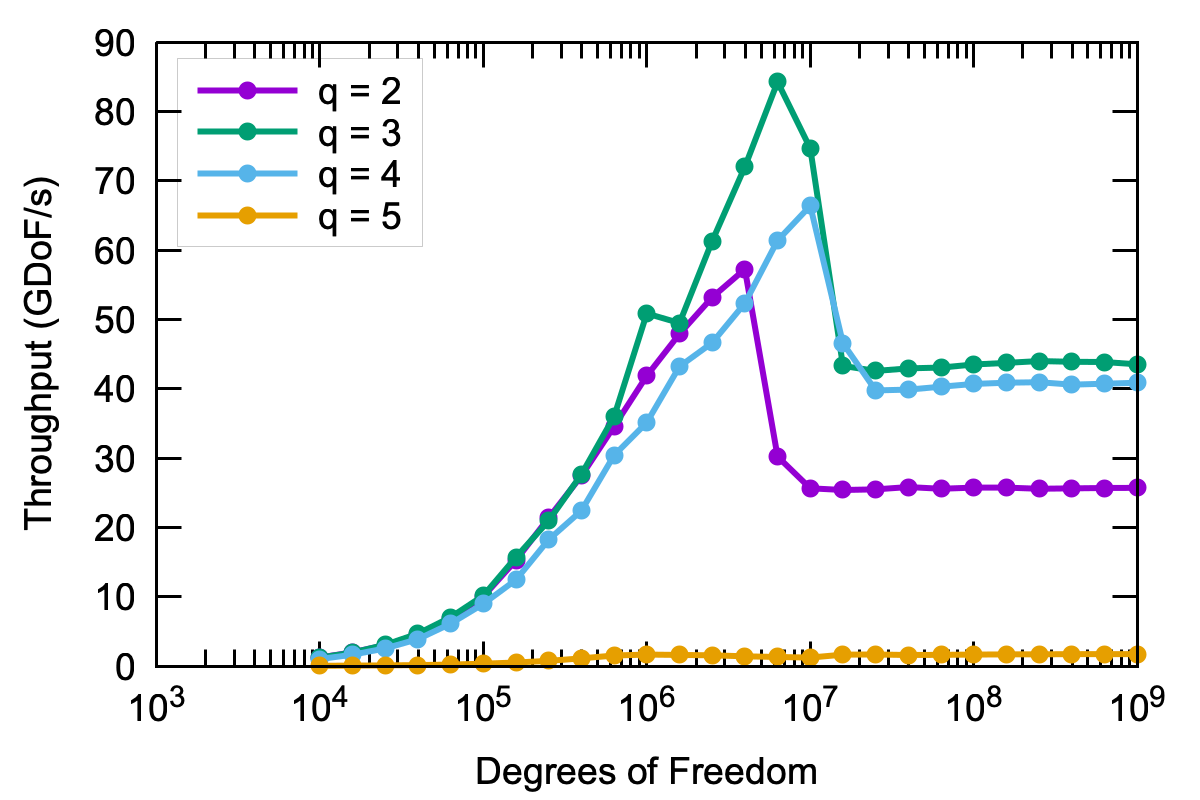
\includegraphics[width=0.8\textwidth]{pvc_openmp} % replace with your filename
  \caption{BK1 performance, Intel Max Series 1550 GPU (Ponte Vecchio).}
  \label{fig:openmp_pvc}
\end{figure}


\begin{figure}[htbp]
  \centering
  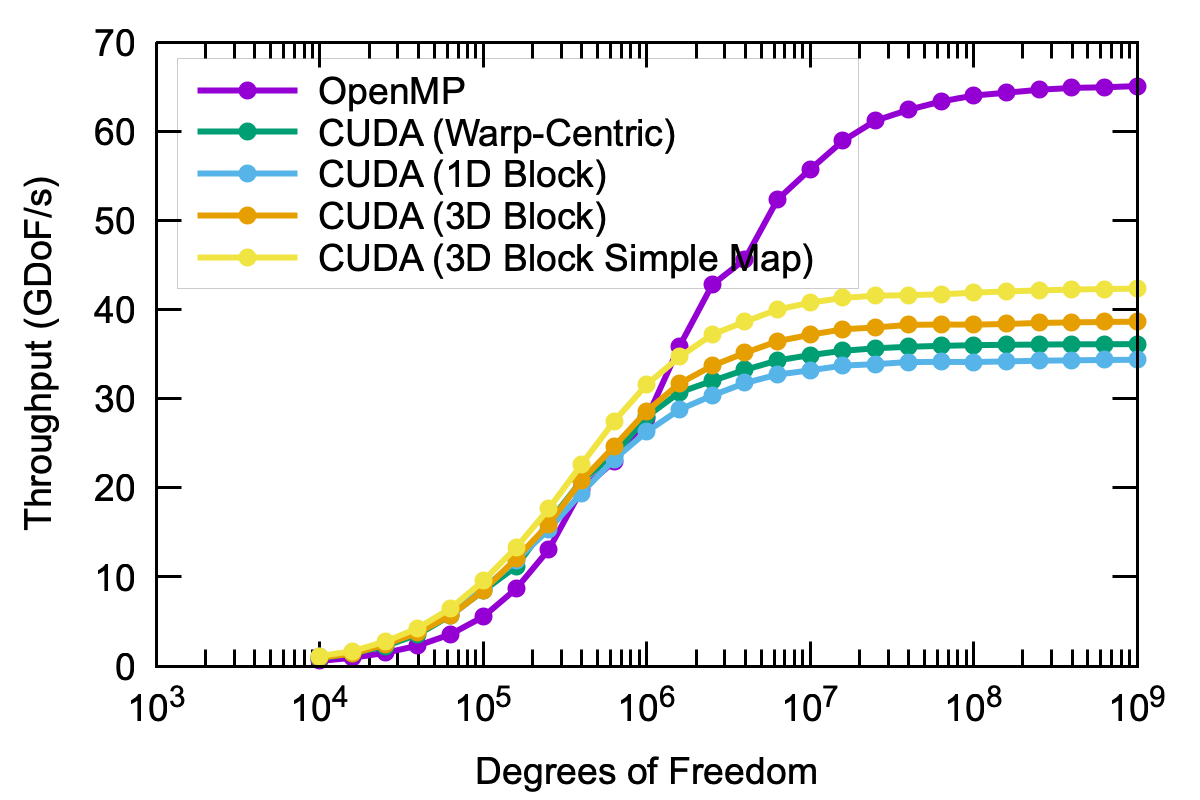
\includegraphics[width=0.8\textwidth]{gh200_templated} % replace with your filename
  \caption{BK1 performance for templated kernel, $q = 4$, Nvidia GH200 (Hopper).}
  \label{fig:openmp_pvc}
\end{figure}

\begin{figure}[htbp]
  \centering
  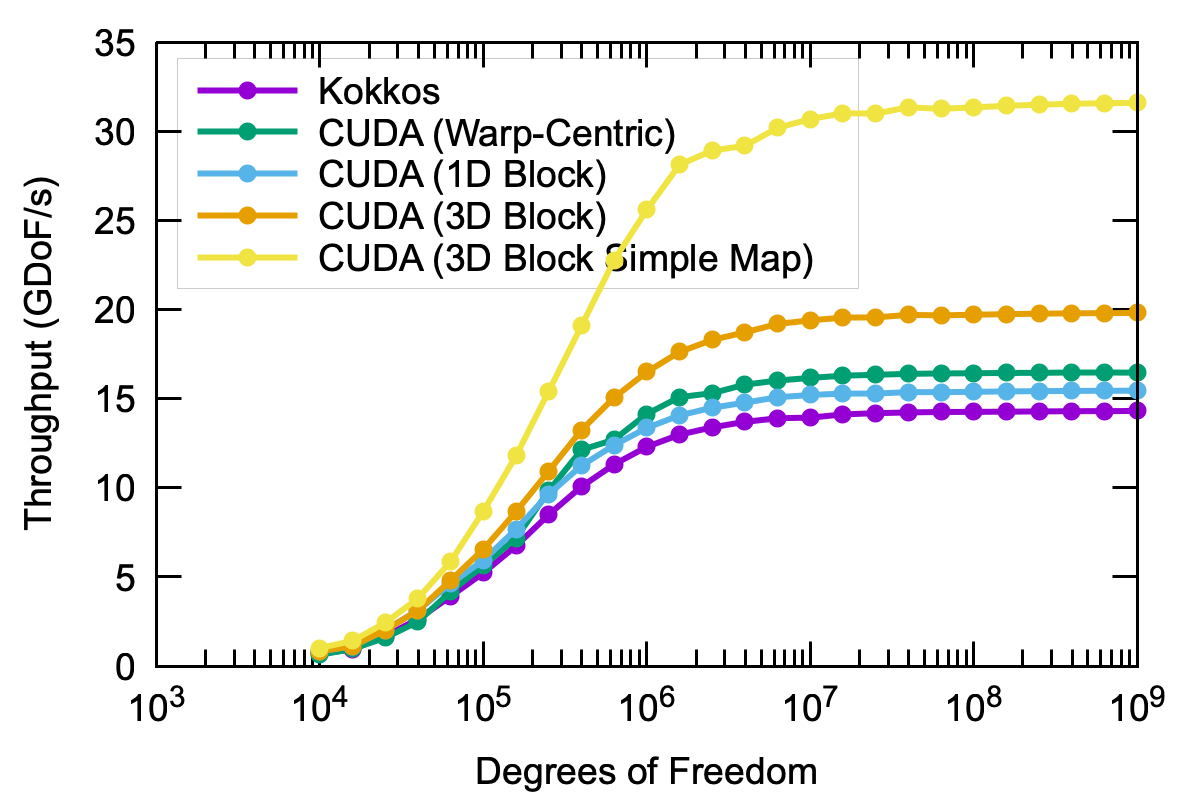
\includegraphics[width=0.8\textwidth]{gh200_variable} % replace with your filename
  \caption{BK1 performance for variable kernel, $q = 4$, Nvidia GH200 (Hopper).}
  \label{fig:openmp_pvc}
\end{figure}
\section{Energy Efficiency}

Implement energy measurement strategies for the main algorithmic ingredients

FIXME: cite Salvatore's work, energy-meter 

\section{Algorithmic development}


\section{Next steps}

\begin{itemize}
    \item TinyTC kernel optimization using fusion and cross-element vectoritation
    \item Use of advanced multigrid solvers and preconditioners
\end{itemize}


\section{Hardware systems}

\begin{center}
    \begin{table}[h!]
    \small
    \caption{GPUs used for evaluation}
    \renewcommand{\arraystretch}{1.25}
    \label{tab:example_table}
    \begin{tabular}{|l|l|l|c|}
    \hline
    \textbf{Column 1} & \textbf{Ampere} & \textbf{Hopper} & \textbf{Ponte Vecchio} \\
    \hline
    execution units & Description & Category & Value \\
    base frequency & Description & Category & Value \\
    SIMT/SIMD width & Description & Category & Value \\
    last level cache & Description & Category & Value \\
    memory bandwidth & Description & Category & Value \\
    \hline
    \end{tabular}
    \end{table}
\end{center}


\end{document}
